\chapter[\paperIVtitle]{\texorpdfstring{%
                \paperIVtitle}{%
                \paperIVtitle}}

\label{ch:digital-twin}
\paperRemark{\paperIVref}


%\theoremstyle{definition}
%\newtheorem{definition}{Definition}[section]


%\section{abstract}
%The digital twin is a rather new industrial control and automation systems concept. While the approach so far has gained interest mainly due to capabilities to make advanced simulations and optimizations, recently the possibilities for enhanced security have got attention within the research community. In this paper, we discuss how a digital twin replication model and corresponding security architecture can be used to allow data sharing and control of security-critical processes. We identify design-driving security requirements for digital twin based data sharing and control. We show that the proposed state synchronization design meets the expected digital twin synchronization requirements and give a high level design and evaluation of other security components of the architecture. We also make performance evaluations of a proof of concept for protected software upgrade using the proposed digital twin design. Our new security framework provides a foundation for future research work in this promising new area.

\section{Introduction}
\label{sec:digital-twin:introduction}

Industrial Automation and Control Systems (IACS) is a very broad term covering everything relating to control, monitoring and production in different industries and encompasses all parts of such systems.

While security for IACS in the past was neglected, in recent years security has obtained a lot of attention in the research community and indeed within the industry. Major security incidents such as the STUXNET worm in 2010 \cite{Falliere2011}, the Shamoon Saudi Aramao spear-phishing attack in 2012 \cite{Leyden2012} and the German steel factory attack in 2014 \cite{Roberts2014} have highlighted the risk of attacks on IACS.  Even if the attacks have been of many different types and origins, they have highlighted the need for enhanced security mechanisms and countermeasures. 

Clear evidence that the industry nowadays takes security issues seriously is the development of best practice security guidelines \cite{Didier2014} and the large number of security standards targeting the IACS domain, like ISO/IEC 27000 series\footnote{https://www.iso.org/isoiec-27001-information-security.html}, the ISA/IEC IEC 62443 series\footnote{ISA, ISA99, Industrial Automation and Control Systems Security, https://www.isa.org/isa99/} and the NIST SP800 series. Among those, IEC 62443 is based on the very general ISO 27000 but specified for the IACS area and also the NIST SP 800-82 \cite{NISTICS2015} in the SP800 series is an IACS standard. In addition, the industrial internet consortium has developed a new security framework \cite{Schrecker2016}. 

New technology trends affect IACS as well as the entire society. Security solutions, security recommendations as well as standards, need to adapt to the new technologies. One clear current trend is the move from legacy ISA-95 to highly distributed and cloud based architectures according to the Industry 4.0 and RAMI 4.0 models \cite{Lee2014}. This transition is demanding in many  ways, one challenge is control and information sharing between production units and cloud based control functions. This constitutes a major security risk and requires careful system engineering not to jeopardize IACS reliability \cite{Delsing2017}. We tackle this general security issue in this paper by looking into the digital twin model as an {\it enabler} for enhanced security when opening up IACS low level control functions and data exchange according to the Industry 4.0 vision. Digital twins and state replication as security enablers were recently proposed by different researchers \cite{Bittion2018},\cite{Eckhart2018}, \cite{Eckhart2018_2}. Previous works have not taken an IACS holistic view and in this paper we look into the problem from a system security point of view. The work is focused on identifying main design driving requirements for a digital twin based IACS security architecture and with special attention to a state synchronization model fulfilling the requirements. Detailed design of the different components and protocols in the architecture as well as formal security analysis of these are left for future work. 
The main contributions of the paper are the following:
\begin{itemize}
    \item We introduce a digital twin IACS adversary model and identify security requirements for this model.
    \item We suggest a novel digital twin based security architecture including a new state replication model.
    \item We evaluate the security of the proposed state replication model as well as present a proof of concept implementation  for a PLC software upgrade case including performance figures.
\end{itemize}
We proceed as follows: we discuss the digital twin model and make basic definitions which we use throughout the paper (\S \ref{Dtwinconcept}), we introduce our adversary model and derive security requirements (\S \ref{dtwinsecurity}),  we suggest a new digital twin security architecture and a novel digital twin design, including a state replication model (\S \ref{architecturedesign}). We make a security analysis of the proposed model and architecture (\S \ref{analysis}) and present a proof of concept implementation, including performance figures (\S \ref{analysis:manufacturing_example}). Lastly we discuss related work (\S \ref{sec:digital-twin:relatedwork}) and conclude (\S \ref{sec:digital-twin:conclusion}).

\section{Digital twin concept, related work and definitions}
\label{Dtwinconcept}
\subsection{Digital twin model and scenario}
\label{Dtwinconcept:model}
The digital twin was according to Grives \cite{Grives2014}, a terminology invented around 15 years ago by John Vickers of NASA and the term was introduced publicly by NASA in 2010 \cite{Shafto2010}. Originally, the concept was used to refer to the digital representation of a product used in simulations software but has been expanded to a concept where not only a physical product is represented in virtual form (software) but each product is directly connected with a virtual counterpart, the digital twin. The general model is depicted in Fig. \ref{figure:digital_twin_model}.

\begin{figure}[ht]
   \centering
    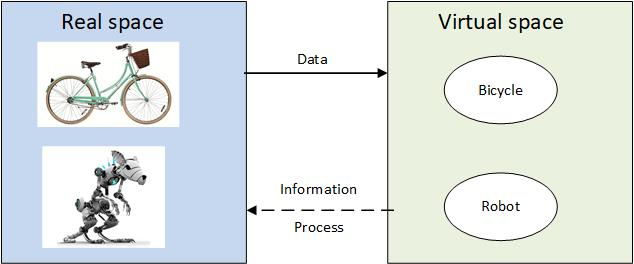
\includegraphics[scale=0.5]{papers/digital-twin/images/FIG1_TII-19-1326}
    \caption{The original digital twin model.}
    \label{figure:digital_twin_model}
\end{figure}

The overall goal with this concept is to be able to closely follow products during production (the physical twin) and simulate the process to adjust the production with results of these simulations. This can be done in real-time or close to real-time to optimize production flows etc. \cite{UHLEMANN2017}. The concept has then been extended to include all units (robot loading stations, conveyor belts etc.) in a production system allowing advanced simulations of a complete manufacturing system and the units involved in an autonomous system \cite{ROSEN2015}. Typically, then the digital twin part is represented and executed on cloud resources \cite{Shahriar2018}. Fig. \ref{figure:digital_twin_cloud} illustrates the overall scenario and model. 

\begin{figure}[ht]
   \centering
    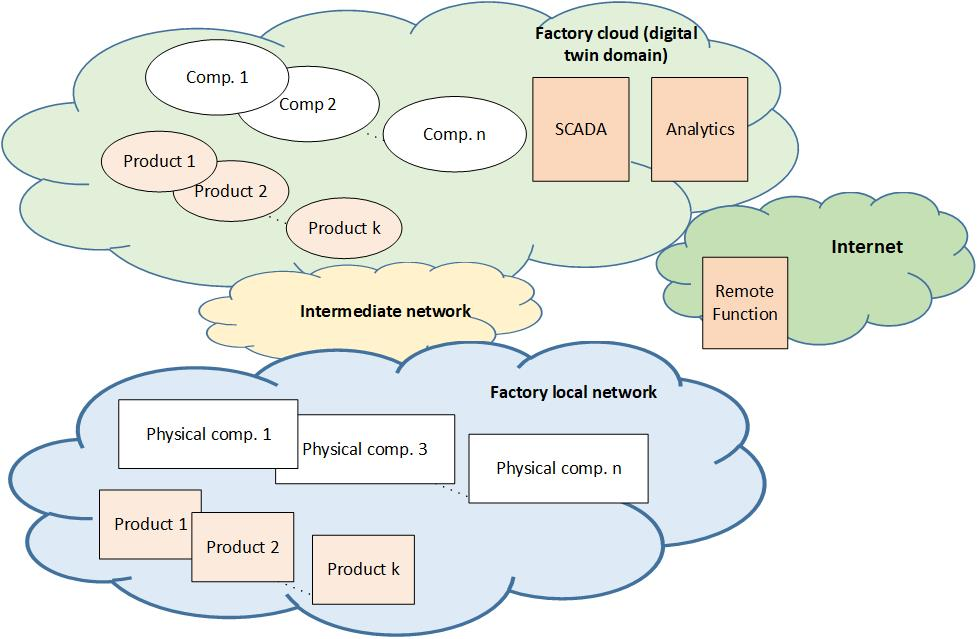
\includegraphics[scale=0.34]{papers/digital-twin/images/FIG2_TII-19-1326}
    \caption{Digital twin cloud system scenario.}
    \label{figure:digital_twin_cloud}
\end{figure}

As can be seen in Fig. \ref{figure:digital_twin_cloud}, according to this model not only are the products themselves reflected as digital twins in the virtual (cloud) domain but also the manufacturing units or what we here refer to as "components". Typical components here are PLCs, historians, sensors, actuators data acquisition units, HMI units etc. Several different models and principles for reflecting such units are possible \cite{Eckhart2018_2}. Here we focus on the network and logical state of a physical twin rather than the physical properties. The definitions and notations we use are introduced in Section \ref{Dtwinconcept:notations} below.

\subsection{Related work}
\label{sec:digital-twin:relatedwork}
Lots of work has been devoted to security in IACS. We will here briefly discuss literature surveys and how our architecture relates to the main security issues previously identified. Next, we will discuss some important previously introduced digital twin models and their relations to our approach. We mainly focus on prior work devoted to digital twin and state replication as enablers for enhanced security. 

Security in IACS in general has been treated in several good surveys \cite{krotofilgollman2013, uchenaEtAl2017}. The work by Krotifil and Gollmann \cite{krotofilgollman2013} focusing on different types of attacks on existing systems but also concluding that most efforts so far have been devoted to IDS. Many existing IDS are compatible with our suggested architecture but it has the benefit that such systems can be deployed in the virtual domain. A very broad systematic overview of security in cyber-physical systems in general (including IACS) is given in by Humayed \emph{et al.} in \cite{HumayedEtAl2017}. The authors identify that major security challenges in IACS are change management (including SW update) as well as the ability to handle legacy systems. Both these issues are tackles with the architecture we proposed in this paper. In addition, as we discussed in the introduction, several existing standards and new standard initiatives, are addressing IACS security in current and future systems. None of the main standardization bodies have so far been working with the digital twin concept as an enabler for enhanced security.

State machine replication has a very long history. Most of the work in this domain has been devoted to \textit{fault tolerance} \cite{Lamport:1978, Schneider1990}. Achieving state replication under the assumption of fault is much more demanding than the security oriented state replication we consider in this paper. We use a different, simpler model, allowing to choose the correct level of state reflection on the digital twin side depending on the security needs (see our state replication model in Section \ref{Dtwinconcept:replication}).  This is justified by the fact that the design goal of a digital twin security system is disparate from a fault tolerance system, as the digital twin cannot replace the physical twin if it fails, but is there to reflect the physical twin and protect it from direct, potential hostile, external interactions.

The digital twin model was first introduced in \cite{Shafto2010}. Lots of work has then been devoted to the topic in resent years and good overview is given in \cite{Negri2017}. The main focus has been on support of health analysis and improved maintenance as well as digitally mirroring the life of the physical entity. We are following the second approach but different from prior the majority of prior art, we are focusing on using the digital twin as an enabler for enhanced security.  

The usage of digital twins for penetrations testing is discussed in a recent work by Bitton \emph{et al.} \cite{Bittion2018}. The author investigate the relation behind a penetration test specification and system realization with focus on system cost optimization. A non-linear programming solution to find an optimal digital twin implementation level needed to perform  certain security analysis tasks is presented. This is an approach that also is applicable to the sub-problem of digital twin realization in a system realizing the security architecture we present in this paper. 

In \cite{Gehrmann2016} the idea of using state synchronization as an IoT security enabler was suggested. However, the model presented in \cite{Gehrmann2016} does not cover state changes on the IoT device side and no complete digital twin state synchronization model is given. Most recently, a digital twin security framework was presented in \cite{Eckhart2018_2} and later extended in \cite{Eckhart2018}. In \cite{Eckhart2018_2}, a digital twin specification principle using Automation ML (AML)\footnote{Actually, automation ML for digital twin modelling was already suggested by Grecyce  \emph{et al.} in 2016 \cite{Greyce2016} but not for any security applications.} was described together with a proof of concept implementation detecting a man-in-the-middle PLC attack. In the follow up work, \cite{Eckhart2018}, also the state replication problem is considered. In this work, a passive state replication model is presented where state updates are purely done based on inputs in the physical domain. The strength with such a model is that it avoids the negative performance impacts of active state monitoring. Inspired by the work in \cite{Eckhart2018_2} and \cite{Eckhart2018}, we have also looked into the problem area of state modeling as security enabler. However, different from the work in \cite{Eckhart2018}, we are looking into how digital twin can protect IACS from {\it external} attacks and not attacks on the factory domain. With this goal, we have proposed a different state propagation model and a security design allowing to  identify attacks at the virtual domain and preventing them for even reaching the physical domain. Furthermore, we have analyzed a complete digital twin system scenario and proposed an overall security architecture for such scenario.

\subsection{Digital twin definition and notations}
\label{Dtwinconcept:notations}
For the purpose of the paper we denote by $u \in U$, a physical twin, where $U$ denotes the set of physical twins in the system. Similarly, we denote by $u' \in U'$, a digital twin where $U'$ is the set of digital twins in the system.  Let then $S_u = \{s_{u0},s_{u1},...,s_{um-1}\}$ and $S_{u'} = \{s_{u'0},s_{u'1},...,s_{u'n-1}\}, m \geq n$, be the finite set of states of $u$ and $u'$, i.e., we assumes that the digital twin always only reflects a {\it subset} of the physical twin states and no states which are not represented in the physical twin.  Furthermore, denote by $I_u = \{i_{u0},i_{u1},...,i_{ur-1}\}$ the set of possible finite inputs to physical twin $u$ and by $I_{u'} = \{i_{u'0},i_{u'1},...,i_{u'd-1}\}$, the set of finite possible inputs to digital twin $u'$. We denote by $s_{u,t}\in S_u$,  the state of physical twin $u$ at clock cycle $t$ and by $i_{u,t}\in I$ the input to $u$ at clock cycle $t$. Similarly, denote by $s_{u',t} \in S_{u'}$,  the state of digital twin $u'$ at clock cycle $t$ and the input to $u'$ at clock cycle $t$ by $i_{u',t} \in I'$. Hence, the initial state of the physical twin is $s_{u,0}$ and the initial state of the digital twin is $s_{u',0}$. Then we can define both the physical and digital twin as finite state machines. We then let $\delta_u: S_u \times I_u \rightarrow S_u$ and $\delta_{u'}: S_{u'} \times I_{u'} \rightarrow S_{u'}$ be the transition functions for the physical and digital twin respectively, i.e. $s_{u,t+1} = \delta_u(s_{u,t},i_{u,t})$ and $s_{u',t+1} = \delta_{u'}(s_{u',t},i_{u',t})$. 

We assume a clock based digital twin state synchronization model where a each clock cycle, $t$, the state of the twins are synchronized with a message exchange starting with a first synchronization message from the $u'$ to $u$ and with a response synchronization message from  $u$ to $u'$. We denote these message as $m_{u'\rightarrow u}(t)$ and  $m_{u \rightarrow u'}(t)$, respectively. These messages are typically not transferred in clear between the twin and intermediate nodes, but in protected/transformed form. We denote protected version of the synchronization messages by $e_{u'\rightarrow u}(t)$ and  $e_{u \rightarrow u'}(t)$.

\section{Adversary model and security requirements}
\label{dtwinsecurity}
Next, using the digital twin model and definition introduced in Section \ref{Dtwinconcept}, we describe a digital twin threat model. Using this threat model we identify security requirements for a digital twin based IACS architecture.
\vspace*{-0.15in}
\subsection{Adversary model}
\label{dtwinsecurity:adversary}
Adversary models for digital twin systems have not been extensively treated in the literature as the concept mostly so far has been used  for production optimization and not security. Certain security aspects regarding using digital twin as security enablers in IACS are considered in \cite{Eckhart2018}  and \cite{Bittion2018}. The authors in \cite{Eckhart2018} consider state replication for active monitoring and intrusion detection while \cite{Bittion2018} consider the problem of penentration testing of IACS with focus on cost optimization for specific security penetration tests (performed on simulated or emulated digital twin or on an acutal physical component in the IACS). However, since these works have very specific security functions goals, they lack adversary model definitions for the digital twin scenario we are considering. Hence, we have developed a new adversary model below. This is {\it not} a generic digital twin adversary model but a model that makes sense in systems with cloud based data sharing and control in IACS. We also give the main motivations for using this rather restrictive adversary model. 

Traditionally, IACS has been separated with firewalls from other networks such as corporate network and the internet.  Several good architectures and recommendations are available  \cite{Schrecker2016}. Here, we assume such principles are deployed and we have adopted an adversary model where we \textit{do not} consider any attacks on the physical twin part or local factory network part of the system but assume these parts can be properly isolated from hostile external networks\footnote{Internal factory network attacks are of course also possible, but we do not consider those in our adversary model.}. 

We assume that the digital twin can run in a separate process even on a third party cloud resource. Then the digital twin can be realized using virtualization techniques where the virtualization is offered on the most suitable level \cite{Smith2005}. Providing strong isolation for virtualization and protection against hostile cloud providers is a very challenging topic which has been widely addressed with several different models and solutions the past ten years \cite{Liu2015, Schuster2015, Paladi2017}. Recent attacks Metldown \cite{Lipp2018} and Spectre \cite{Kocher2019} have shown that one cannot even trust the fundamental hardware functions needed for secure isolation currently in use. However, the security with respect to secure execution environment for virtualized systems is steadily improving and we will for simplicity in this paper disregard attacks on the isolation properties of the digital twin and assume that a secure execution environment and data storage is provided for the digital twin in the system.

We adopt the Dolev-Yao model \cite{Dolev1981} and assume that the attacker can influence the system in all other aspects including the following capabilities of the adversary:
\begin{itemize}
    \item The attacker is able to intercept, modify and replay all communication from the physical domain to the digital domain and vice versa.
    \item The attacker is able to launch input attacks by sending arbitrary messages to a digital twin and input requests, i.e. he or she can choose to send arbitrary input from the set $I_{u'}$ to the digital twin $u'$.
    \item The attacker is able to launch intercept, modify and replay any information sent between digital twins or between digital twins and other units executing in the virtual domain.
\end{itemize}

\subsection{Security definitions}
Next, we give basic security definitions. The basis of the new security architecture is the introduction of state replication between the physical and digital twin. An expectation from such model from \emph{robustness} perspective is that the synchronization is accurate over all system states and inputs. The synchronization consistent expectation is fundamental for deploying the architecture and very different from architectures introduced in the literature before. The main reason why consistency is important is that without it, one cannot rely on that all system changes in the digital twin part are correctly propagated to physical part of the system and vice versa, which will make it impossible to use the model in practise as the system behaviour would be unreliable. Hence, even if the synchronization consistency not is a pure security requirement, it is fundamental for the proposed architecture and we make a precise definition of synchronization consistent ency. It is also important to notice that one would expect from a specific design and implementation of our architecture to provide the synchronisation consistency property also under attack conditions. Hence, it is important to introduce a proper definition also in this regard.

Another fundamental, pure security expectation, with respect to the synchronization is the confidentiality and integrity of the synchronization process as such. Hence, we also provide precise definitions for these two aspects.  Apart from these definitions, we adopt widely used computer and communication security definitions \cite{Stallings2014}.

\label{dtwinsecurity:defintions}
\theoremstyle{definition}
\begin{definition}
\label{dtwinsecurity:consistent}
A digital twin system is \emph{consistent} if there exist functions $\forall u \in U,f_u: S_u\rightarrow S_{u'}$such that the following is true:
\begin{eqnarray}
    \forall s \in S_u, f_u(\delta_u (s,\emptyset))  & =  &\delta_{u'}(f_u(s),\emptyset),\label{dtwinsecurity:const1}\\
	s_{u',0} & = &f_u(s_{u,0}). \label{dtwinsecurity:const2}
\end{eqnarray}
\end{definition}

This definition reflects the requirement that when the digital twin starts in a state consistent with the staring state of the physical counterpart and whenever neither the physical twin nor the digital twin receive any input, they are both always transitioned to states that are consistent. i.e. the physical to digital twin state mapping agree with the state of the digital twin.

\begin{definition}
\label{dtwinsecurity:confidentiality}
A digital twin system synchronization protocol provides \emph{confidentiality protection} if an adversary, who observes information, $e_{u'\rightarrow u}(t)$ and $e_{u\rightarrow u'}(t))$, sent from the digital twin and from the physical twin respectively at time $t$,  cannot execute any attack, $A$, that in polynomial time will allow the attacker to distinguish the state of the physical twin from any randomly selected state, i.e., after execution of $A$, the following is true: 
\begin{eqnarray}
    \forall s \in S_u,  Pr(s_u = s|e_{u'\rightarrow u}(t), e_{u\rightarrow u'}(t)) = Pr(s_u = s) \label{dtwinsecurity:eqconfidentiality}
\end{eqnarray}
\end{definition}

\begin{definition}
\label{dtwinsecurity:synchprot}
A digital twin system synchronization protocol provides \emph{synchronization protection} if the adversary cannot execute any attack replacing message exchange $e_{u'\rightarrow u}(t)$ with $e'_{u'\rightarrow u'}(t)$ and/or replacing $e_{u\rightarrow u'}(t)£$ with $e'_{u\rightarrow u'}(t)$ which will be accepted by $u$ and $u'$ and making the twins out of synchronization, i.e.  $f_u(s_{u,t}) = s_{u',t}$ is always true after successful synchronization independent of adversary substitution choices\footnote{This definition does {\it not} take a DoS attack into account and assumes that the synchronization messages arrives at each time slot.}.
\end{definition}

\begin{figure}[th]
\hspace*{-0.2in}
   \centering
    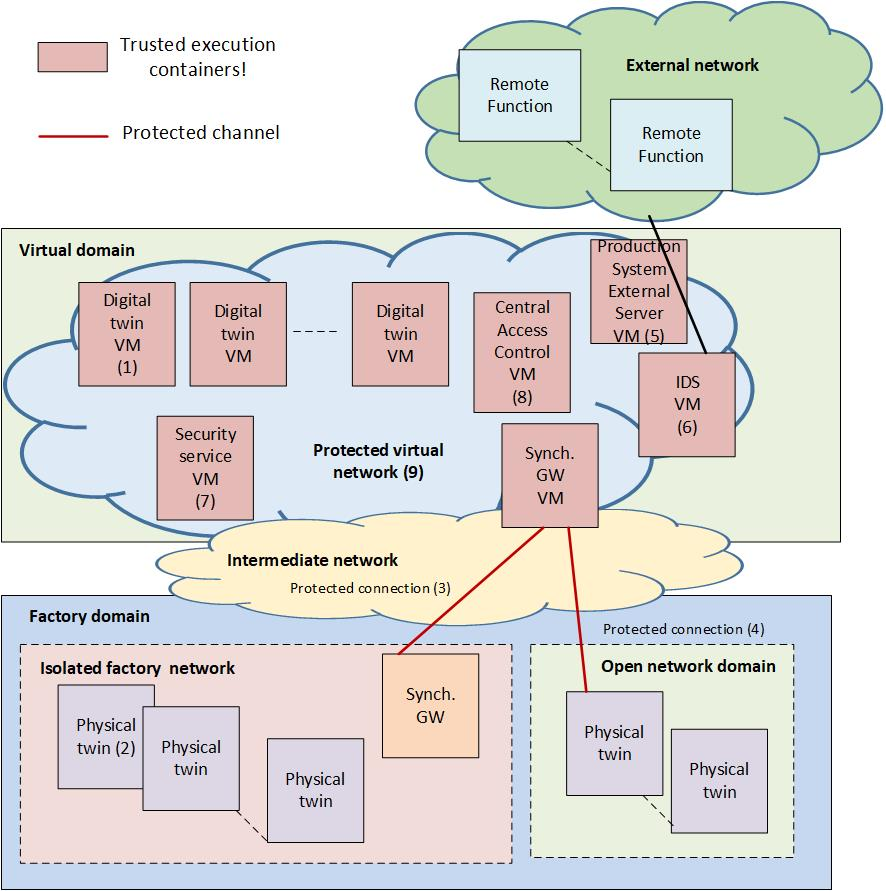
\includegraphics[scale=0.35]{papers/digital-twin/images/FIG3_TII_191326}
    \caption{Security architecture overview.}
    \label{figure:security_architecture}
    
\end{figure}
\vspace*{-0.2in}
\subsection{Requirements}
\label{dtwinsecurity:requirements}
We have used the previously presented adversary model and security definitions to identify a set of system security, performance and accuracy requirements. This is not an exhaustive list but the major identified system architecture requirements.
\begin{labeling}{R6.}
\item [R1.] \textbf{Synchronization security:} We require the digital twin state replication model and protocol to be consistent (Definition \ref{dtwinsecurity:consistent}), provide confidentiality protection (Definition \ref{dtwinsecurity:confidentiality}) and synchronization protection (Definition \ref{dtwinsecurity:synchprot}).
\item[R2.] \textbf{Synchronization latency:} The synchronization message exchange must not cause any delays which prevent time critical control functions to be propagated to from the physical to the digital twin. The precis requirements are application dependent.
\item[R3.] \textbf{Digital twin external connections protection:} All connections between the digital twin and the external entities must be authenticated. According to the adopted adversary model, we assume each digital twin to run in a protected execution environment but all request external to this environment must be properly authenticated and all information sent from the digital twin to external trusted parties must be confidentiality and integrity protected. 
\item[R4.] \textbf{Access control:} The digital twin itself or a secure entity in direct connection with the digital twin needs to make sure access control is applied on on all incoming requests.  This includes request and information exchange with external parties as well as information exchange with other digital twins. 
\item[R5.] \textbf{Software security:} The physical twin software must always be in a trustworthy state. This implies that the physical twin must be protected from installation of harmful software. Mechanisms shall be in place to recover the system in case of zero-days attacks on the physical twins.
\item[R6.]\textbf{Local factory network isolation:} The local factory network shall not accept any connection requests except for protected synchronization requests with the digital twin (see R1 above).  Physical twins should be protected from DoS attacks through boarder unit such as a gateway or firewall making sure that only protected synchronization requests reach a physical twin and no other outside traffic.
\item [R7.] \textbf{Digital twin Denial-of-Service (DoS) resilience:} The digital twin must be protected from DoS attacks such as network flooding or distributed DoS directly targeting a digital twin. Proper DoS filters and router configurations must be deployed in the factory cloud domain to prevent or limit the DoS possibilities of the attacker. At the same time, filters and router policies must not prevent synchronization exchanges to reach the digital twins in the system.
\end{labeling}

\section{A digital twin based security architecture and state replication design}
\label{architecturedesign}

\subsection{Security architecture}
\label{dtwinsecurity:architecture}
We now have the definitions and requirements in place to define a generic digital twin security architecture. Fig. \ref{figure:security_architecture} gives a high-level picture of the proposed architecture. We have here focused on the main security properties and entities in the system. This is {\it not} a complete design in all details but a high level design including main components and their roles in the architecture. We verify the key digital twin design of it in our proof of concept evaluation but leave detailed design and evaluation of other components for future work.

A basic security assumption in this architecture is the possibility to launch digital twins as well as security services in \textit{trusted execution containers} as Virtual Machines (VMs) on suitable cloud resources. The architecture is completely agnostic on the virutalization technique used for this or on which actual level the vitalization is applied  \cite{Smith2005} \cite{Gehrmann2016}. However, the architecture requires the virtualization technology to provide trusted execution in the sense that different VMs are strongly isolated from each other and that they have access to protected volatile and non-volatile storage.

Using the numbering introduced in Fig. \ref{figure:security_architecture}, we discuss the different properties of the components in the architecture below.
\subsubsection{Digital twin component} The digital twin component is running as a VM in an isolated environment. An overview picture of the main logical functions of the twin is given in Fig. \ref{figure:dtwin_security_architecture}. The core functionality of the digital twin is the actual simulation of the physical counterpart. Only two direct external network interactions are allowed: the synchronization (which occurs over the synchronization GW) and the exchange with external requests and responses. This takes place either through the cloud server which takes \textit{all} incoming requests and responses from external entities or directly to other digital twins or back-end components. The virtual domain external connections are protected through the cloud Virtual Private Network (VPN) (see Section \ref{dtwinsecurity_secarch_VPN}). The state of the digital twin is \textit{exported} directly to a \textit{common} (for several digital twins in a system) security analysis component (see also Subsection \ref{dtwinsecurity:security_analysis}). Also the intermediate state, $\hat{s}_{u'}$, is exposed to an analyzer in this way. This implies that an external analyzer can have access (if allowed by the access policy) to all digital twin states in the system. This in turn allows \textit{abortion} of state propagation in case of detection of a fatal security issue by the external analyzer. The digital twin has access to a secure clock, $t$, for precise synchronization operations with the physical twin.  The actual state propagation design we use is described in Section \ref{Dtwinconcept:replication}.

\begin{figure}[ht]
   \centering
    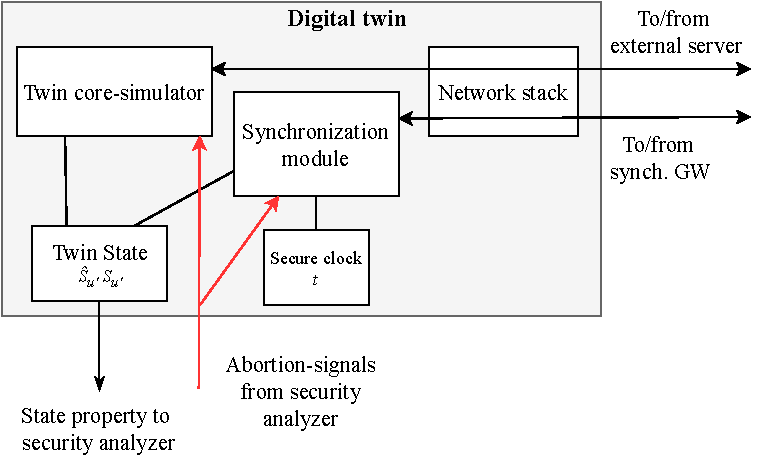
\includegraphics[scale=0.65]{papers/digital-twin/images/FIG4_TII-19-1326}
    \caption{Digital twin main functions}
    \label{figure:dtwin_security_architecture}
\end{figure}

\subsubsection{Physical twin component}
An overview picture of the main logical functions of the physical twin is given in Fig. \ref{figure:phytwin_security_architecture}. Similar to the digital counterpart, the physical twin executes the defined synchronization protocol. Depending on if the physical twin actually has network connectivity or not, it might run the synchronization itself or it is done through a ''measurement unit''\footnote{For a physical twin that is in production, it could be that it has no program execution capabilities, but its state is only measured through external sensors for instance.}. A physical twin deployed in an isolated factory network will only exchange synchronization information with a dedicated synchronization GW on the same network. On the other hand, a single deployed physical twin outside such a network will need to directly exchange synchronization information with the synchronization GW in the virtual domain and needs access to the key material needed for such secure interactions. The physical twin will apart from this, not need any specific security adaptations at all. The state propagation design applicable to the physical twin is described in Section \ref{Dtwinconcept:replication}.

\begin{figure}[ht]
   \centering
    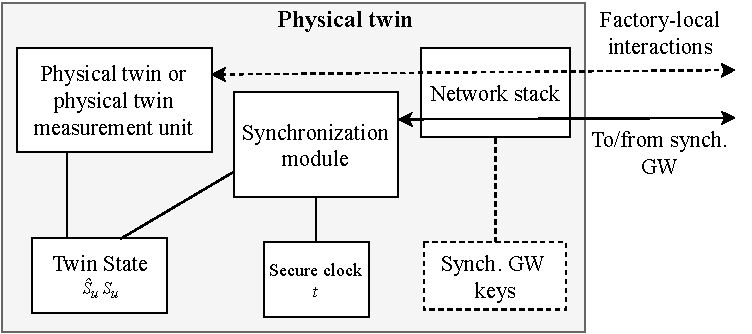
\includegraphics[scale=0.65]{papers/digital-twin/images/FIG5_TII-19-1326}
    \caption{Physical twin main functions.}
    \label{figure:phytwin_security_architecture}
\end{figure}

\subsubsection{Protected connection between synchronization gateways} 
\label{dtwinsecurity:arch_protected_connection}
The connection between the synchronization GW on the local factory and the virtual domain is protected through a secure channel. We have chosen this principle instead of end-to end synchronization protection as we assume it will be possible to deploy synchronization GWs in trusted containers in the virtual domain. Standard IPsec \cite{Kent2005} VPN or a TLS/DTL channels \cite{Dierks2008} \cite{rfc6347} are assumed. A major advantage with such solution from security management point of view is that this allows a \emph{single} security relation between the physical and digital domain. Such single relation is very easy to maintain from security perspective. For instance, can a pres-shared key TLS or DTLS relation for instance be used. This can be compared to a situation where external entities are allowed to directly connect to the physical domain. In such situation, each external connection would need a separate security relation with the physical domain. Now, such relations are instead moved to the digital domain, where the security risk is much lower and where it is much less complex to handle such relations from a security configuration management point of view.
\subsubsection{Protected connection from isolated physical twin to synchronization gateway}
A physical twin not deployed in a protected local factory network, needs to directly connect to the synchronization GW in the virtual domain. This connection then obviously needs to be confidentiality and integrity protected using a suitable secure channel (see Section \ref{dtwinsecurity:arch_protected_connection}).
\subsubsection{Production system external server}
The architecture assumes all external requests arrives in the virtual domain, i.e. external input to digital twin $u'$ from the set $I_{u'}$ arrives to the production system external server prior to (potential) being forwarded to the digital twin $u'$. Similar responses from a digital twin are routed through this sever as well. This allows advanced network filtering at a single point and avoids having such functionality duplicated at each digital twin virtual instance\footnote{Recall that in our adversary model we assume all inputs to a \textit{physical} twin to be trustworthy and not subject to direct security analysis}.
\subsubsection{Intrusion Detection System (IDS)}
State-of-the art IDS are best deployed at the boarder to the internet \cite{Kruegel2002}. We adopt this principle and assume the actual intrusion analysis to be done by a VM with direct access to the external network interface traffic. 
\subsubsection{Security analysis service} \label{dtwinsecurity:security_analysis}
The core benefit from a security perspective with a digital twin model like the one we have defined, is the possibility to do security analysis directly on the digital twin state and even on the states of a whole family of digital twins. By letting the analyzing engine having access not only to the final states, but also intermediate states, i.e. the $\hat{s}_{u'}$ states in the system, it is possible for a security analysis function to detect harmful state transitions (prior to the state propagating to the physical twin) and take direct action in the digital domain (see also Fig. \ref{figure:dtwin_security_architecture}).
\subsubsection{Central access control}
By letting all external digital twin access be subject to a single point access control, system wide policies can easily be deployed in the system.  Advanced security policies can be defined through standard access control frameworks such as Extensible Access Control Markup Language (XACML) \cite{Rissanen2013}. In order to allow direct interaction between digital twins, this is preferably combined with component local policy enforcement through tokens issued at the central access control entity using standard tokens such as SAML \cite{Campbell2015} or OAuth \cite{Hardt2012}. 
\subsubsection{Protected virtual network}
\label{dtwinsecurity_secarch_VPN}
Most cloud providers offer network isolation between VMs launched on cloud resources\footnote{https://docs.aws.amazon.com/vpc/index.html\#lang/en\_us}\footnote{https://docs.microsoft.com/en-us/azure/virtual-network/virtual-networks-overview}. Even if we have not assumed all trusted execution services to be deployed as complete, "traditional" VMs in the virtual domain, higher layer VMs can be launched on such VMs allowing re-use of standard principles for network isolation. There are also other, non-provider dependent solutions to achieve this \cite{Li2010}.

\subsection{State replication model and design}
\label{Dtwinconcept:replication}

Several different state replication principles for digital twins are possible. Recently, a specification-based state replication model for digital twins was proposed \cite{Eckhart2018}. We have adopted a similar physical and digital twin state transition model. However, the state replication design in \cite{Eckhart2018} is built upon measurement of input values and that the physical and digital twin runs {\it functional identical programs} or what the authors refers to as ''passive state replication''. This is an approach that is efficient if the main purpose of the design is to evaluate security breaches stemming from the physical domain. Instead, we in our security architecture use the digital twin as a ''guard'' against all, potential hostile, {\it external} stimuli on the physical domain. Hence, even if demanding from real-time perspective, we instead have adopted a direct state replication or what the authors in \cite{Eckhart2018} refers to as ''active monitoring''. This different security goal and approach also allow us to abandon the functional identical program requirements. 
We assume a model, where the physical and digital twin are synchronized on regular basis. Without loss of generality, we assume that a synchronization is done at each clock cycle. Let $z_u:S_u \times S_{u'}\rightarrow S_u$ be a synchronization function and $h_u: S_u \rightarrow S_{u'}$ a physical to digital state mapping function for twin $u$. The complete synchronization (including the twins state updates) then consists of the following operations:
\vspace*{-0.08in}
\begin{eqnarray}
\hat{s}_{u,t+1} & = & \delta_u(s_{u,t},i_{u,t}) \label{physprelsynch}, \\
\hat{s}_{u',t+1} &=& \delta_{u'}(s_{u',t},i_{u',t}) \label{digprelsynch}, \\
	s_{u,t+1} & = & z_u(\hat{s}_{u,t+1},\hat{s}_{u',t+1}) \label{digtsynch}, \\ 
	s_{u',t+1} & = & h_u(s_{u,t+1}). \label{physdsynch}
\end{eqnarray}
This synchronization model works such that the physical and digital twin treat their respective inputs independently. We assume that the input will change the state of the (respective) twins independently, and then at the next time slot, they will synchronize their states to make them consistent considering the inputs received before last synchronization. 

The choice of the functions $z_u$ and $h_u$ will depend on the digital twin model and the exact relation between the physical and digital twin. Many different models are possible. For the purpose of this paper, we choose a simple twin model but still a model allow to cover several important security cases as we show in Section \ref{analysis:manufacturing_example}. Denote by  $S_u = S1_u \bigcup S2_u \bigcup S3_u$, we then make the following assumption:  $S1_u \bigcap S2_u = S1_u \bigcap S3_u = S2_u \bigcap S3_u = \emptyset$. Let $S_{u'} = S1_{u'} \bigcup S2_{u'}$ and we assume that $S1_{u'} \bigcap S2_{u'} = \emptyset$. Then we can write the state of the physical twin as $s_u = (s1_u,s2_u,s3_u)$ and the state of the digital twin as $s_{u'} = (s1_{u'},s2_{u'})$. We then apply the following restrictions:
\begin{eqnarray}
 S2_u   & = &  S1_{u'}, \label{arch:s2eq}\\
 S3_u   & = & S2_{u'} \label{arch:s3eq}, 
 \end{eqnarray}
 \begin{eqnarray} 
 \forall s_u \in S_u,  \forall i_u \in I_u, \delta_u(s_u,i_u)   =  \nonumber \\  
 = (\delta1_u(s_u,i_u), \delta2_u((s2_u,s3_u),i_u), s3_u), \label{arch:phystransrestric}\\
  \forall s_{u'} \in S_{u'}, \forall i_{u'} \in I_{u'},  \delta_{u'}(s_{u'},i_{u'})   =  \nonumber \\  
 =   (s1_{u'}, \delta2_{u'}(s_{u'},i_{u'})) \label{arch:digtransrestric}
\end{eqnarray}

In addition, we let
\begin{eqnarray}
 s_{u',0}  =  (s1_{u',0},s2_{u',0}) = (s2_{u,0},s2_{u',0}), \label{arch:digsynchstart}\\
 s_{u,0}  =  (s1_{u,0},s2_{u,0},s3_{u,0}) = (s1_{u,0},s2_{u,0},s2_{u',0}) \label{arch:physsynchstart}
\end{eqnarray}

With these restrictions, we then let $z_u(\hat{s}_{u,t},\hat{s}_{u',t}) = (\hat{s}1_{u,t}, \hat{s}2_{u,t}, \hat{s}2_{u',t})$ and
\begin{equation}
h_u(s_{u,t+1})
= \left \{ \begin{array}{ll}
(s2_{u,0},s3_{u,0})   & \mbox{if $t<0$} \\
(\hat{s}2_{u,t+1}, \hat{s}2_{u',t+1}) & \mbox{otherwise}  \end{array} \right.
 \label{arch:zerostate}
\end{equation}

To send the \textit{complete} state at each synchronization occasion is very inefficient. Instead, the state changes (deltas) are calculated:
\begin{eqnarray}
m_{u'\rightarrow u}(t) & = & \Delta_{\hat{s}_{u'}} =  \textrm{Diff}(\hat{s}_{u',t+1},s_{u',t}), \label{arch:firstdelta} \\
m_{u \rightarrow u'}(t) & = & \Delta_{s_{u'}} = 
\textrm{Diff}(\hat{s}2_{u,t+1},s2_{u,t}), \label{arch:seconddelta}
\end{eqnarray}
This implies that the digital twin calculates a first delta, $\Delta_{\hat{s}_{u'}}$, and sends it to the physical twin. This delta is then used by the physical twin to reconstruct $\hat{s}_{u',t+1}$, which is the input to the $z$ function, i.e. equation (\ref{digtsynch}). Next, the physical twin calculates the ''return delta'', $\Delta_{s_{u'}}$ , that is sent back to the digital twin.   The principle is illustrated in Fig. \ref{figure:digital_twin_synch} below. Observe, that we here only illustrate the synchronization information exchange and not the protection of the synchronization messages as such. The protection principles we apply was described in Section \ref{dtwinsecurity:architecture}.

\begin{figure}[ht]
   \centering
    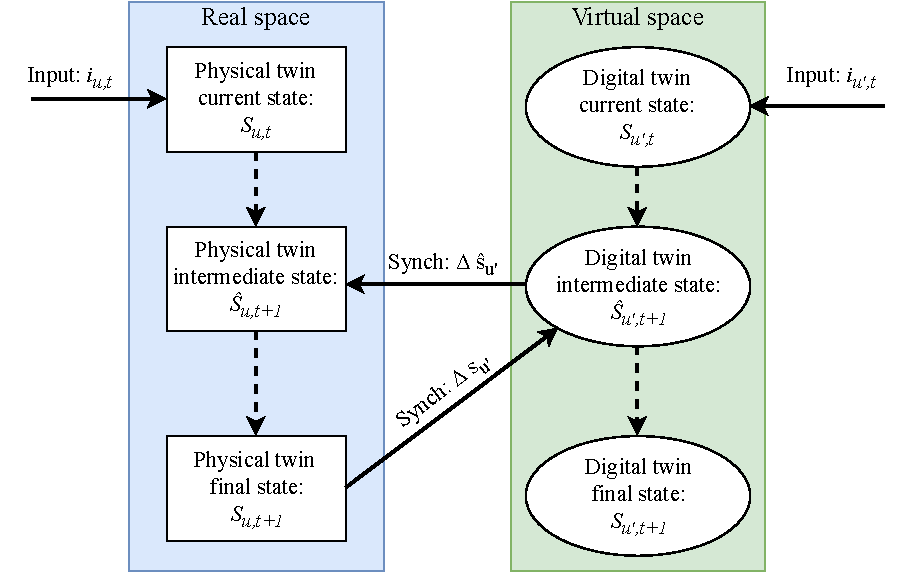
\includegraphics[scale=0.55]{papers/digital-twin/images/FIG6_TII-19-1326}
    \caption{Synchronization principle.}
    \label{figure:digital_twin_synch}
\end{figure}

It is important to notice from real-time and communication overhead perspectives that when no input is received neither on the physical or digital side, there is no need for the twins to exchange any deltas. This is true given a consistent digital twin system synchronized with accurate clocks.

\section{Security analysis}
\label{analysis}
Next, we analyze the proposed framework from security and performance perspectives. We here mainly focus on the synchronization security characteristics. We also give arguments regarding how the proposed architecture meets the other security requirements listed in Section \ref{dtwinsecurity:requirements}. As the architecture in many aspects only include a high level design, we here postpone detailed security evaluation of these aspects to future work and for specific implementation designs. 
\subsubsection{Synchronization security}
%\newtheorem{prop}{Proposition}
\begin{prop}
\label{analysis:synchsec}
The digital twin synchronization model and protocol is consistent.
\end{prop}
\begin{proof}
Let:
\begin{equation}
f_u(s) = f_u((s1,s2,s3)) = (s2,s3). \label{fdef}
\end{equation}
From (\ref{arch:physsynchstart}) we have that $s_{u,0} = (s1_{u,0},s2_{u,0},s2_{u',0})$ and from (\ref{arch:digsynchstart}) and (\ref{arch:zerostate}), it then follows that $f_u(s_{u,0}) = h_u(s_{u,0}) =  (s2_{u,0},s3_{u,0}) = (s1_{u',0},s2_{u',0}) = s_{u',0}$, which fulfils condition (\ref{dtwinsecurity:const2}).

\noindent
Now, using the assumptions (\ref{arch:s2eq}),  (\ref{arch:s3eq}), (\ref{arch:phystransrestric}) and (\ref{arch:digtransrestric}), let:

$\hat{\delta}_u(s_u,i_u) = (\delta1_u(s_u,i_u), \delta2_u((s2_u,s3_u),i_u), \delta2_{u'}((s2_u,s3_u),\emptyset)$.

\noindent
Then, it follows from (\ref{fdef}),

$f_u(\hat{\delta}_u(s_u,\emptyset)) = (\delta2_u((s2_u,s3_u),\emptyset), \delta2_{u'}((s2_u,s3_u,\emptyset))$. 

\noindent
Similar, let:
$\hat{\delta}_{u'}(s_{u'},i_{u'}) = (\delta2_u((s1_{u'},s2_{u'}),\emptyset),\delta2_{u'}(s_{u'},i_{u'}))$. 

\noindent
Then by direct calculation:

$\hat{\delta}_{u'}(f_u(s_u),\emptyset) = \hat{\delta}_{u'}((s2_u,s3_u),\emptyset) = $ 

$(\delta2_u((s2_u,s3_u),\emptyset),\delta2_{u'}((s2_u,s3_u),\emptyset)) = f_u(\hat{\delta}(s_u,\emptyset))$.

\noindent
 By then letting the state $s_u$ taking any value in $S_u$, it follows that also condition (\ref{dtwinsecurity:const1}) is fulfilled.
\end{proof}
\begin{prop}
\label{analysis:proofconfidentiality}
If the secure channel used for communication towards and between synchronization GW in the architecture provides confidentiality, the digital twin synchronization design also provides confidentiality.
\end{prop}
\begin{proof}
According to our attacker model, an adversary can intercept any message sent from the digital twin to the synchronization GW in the virtual domain or any messages sent between synchronization GWs. He or she might also intercept message sent from physical twins towards the GW deployed in the virtual domain. The attacker has no other option to intercept any synchronization information.
According to (\ref{arch:firstdelta}) and (\ref{arch:seconddelta}), at each clock cycle, one delta message is sent from the digital twin towards the physical twin and a replay delta message is sent in return. An adversary has two options to intercept the first message, $e_{u'\rightarrow u}(t)$; Either he or she intercept it when it is sent from the digital twin the synchronization GW in the virtual domain {\it or}\ when it is forwarded from the synchronization to the GW in the factory domain (or physical twin in the second option). As long as both these channels provide confidentiality the attacker will not get any information on $s_u$. As the return message follows the very same path, the also the return message, $e_{u \rightarrow u'}(t)$ , will have the very same protection and equation (\ref{dtwinsecurity:eqconfidentiality}) is fulfilled.
\end{proof}
\begin{prop}
If the secure channel used for communication towards and between synchronization GW in the architecture provides integrity and replay protection, the digital twin synchronization design also provides synchronization protection.
\end{prop}
\begin{proof}
According to Proposition \ref{analysis:synchsec} the proposed synchronization model is consistent and consequently if no input is received on neither the digital nor physical twin, $h_u(s_{u,t+1}) = s_{u',t+1}$. Furthermore, if the synchronization messages also arrives unmodified equation (\ref{physdsynch}) guarantees that $h_u(s_{u,t+1}) = s_{u',t+1}$ holds also in this case. Hence, the only option for an attacker would be to modify any messages $e_{u'\rightarrow u}(t)$ or $e_{u\rightarrow u'}(t))$. In analogue with the proof of Proposition \ref{analysis:proofconfidentiality}, if the used secure channels provides integrity and replay protection, such modification will be detected and a modified or replayed message will be rejected.  
\end{proof}
\subsubsection{Latency}
The architecture as such does not make any direct assumption regarding the synchronization real-time behaviour. Depending on the specific IACS application, the networks must be chosen and configured accordingly. Similarly, the synchronization GW must be implemented on platforms powerful enough to fulfill real-time requirements. For some applications, deploying the virtual domain on an edge cloud \cite{Delsing2017} can be used to meet R2.  
\subsubsection{External connections}
The architecture assumes all external connection to be intermediates by the external server entity at the boarder of the external network. The external server will only accept authenticated requests. Furthermore, the final hop for the external server to the digital twin runs through the virtual domain VPN. This, if properly implemented, implies that the system fulfills the requirement R3. 
\subsubsection{Access control}
According to the proposed security architecture, the centralized access control VM deployed in the virtual domain makes sure all access requests towards the digital twin are properly authorized. Access control enforcement then takes place at the digital twin VM. This means that the main building blocks are included to fulfil R4. However, the actually authorization and access control mechanisms which are supported are subject to detailed design, which have been left for future work.
\subsubsection{Software security}
The software state of the physical twin can be replicated to the digital counterpart. A security service with direct access to the twin state can be launched. This service then controls the physical twin software state and upgrade. This is a very efficient way to both monitor the SW status and control upgrades as we show with the experimental evaluation in Section Section \ref{analysis:manufacturing_example}. Even if this is an important step to meet R5, further SW monitoring tools needs to be deployed in the system to give the wanted software security level.  
\subsubsection{Network isolation and DoS resilience}
The architecture adopts best practise for factory network isolation \cite{NISTICS2015} to meet R6. In addition, external interaction with the factory domain is only possible indirectly through the protected synchronization. All direct requests towards digital twin are subject to IDS and filtering and additional security protection mechanism can be launched as security service VMs in the virtual domain. With proper design and implementation, such measures will provide network isolation and DoS resilience as required by R7.

\section{Proof of concept and performance evaluation}
\label{analysis:manufacturing_example}
In order to test the feasibility of the proposed architecture and approach, we have implemented a low complexity system with digital twins using our proposed state synchronization protocol. Our main goal here is to get an impression of how the proposed synchronization framework, which is the fundamental basis of the proposed architecture, affects the production units in the system as well as the bandwidth consumption\footnote{We recall that the synchronization including the protection of the synchronization is the only parts of the architecture that directly affects the production domain.}. It was argued in \cite{Eckhart2018} that direct state synchronization or what the authors refer to as ‘’active monitoring’’ is not feasible in real-time critical systems due to large bandwidth overhead. While we argue that this is not the case for low complexity digital twin state models and for moderate synchronization frequencies, we are interested to measure the production unit actual computation and bandwidth overhead in a real system. To make the evaluation feasible, we here focus on the {\it first three} components in the architecture in Fig. \ref{figure:security_architecture}.  We have implemented a simple manufacturing scenario, as seen in Fig. \ref{figure:setup} consisting of a PLC unit, $u_1$, controlling an industrial process. In addition, we have a software upgrade server, $u_2$, holding software upgrade information, that is deployed in the factory local network. The PLC and the upgrade server are reflected as digital twins: $u'_1, u'_2$. The goal with introducing the virtual domain is to allow secure software control and upgrade of the production system units. To facilitate this, the software state and software control state are replicated to the digital twin domain. 

It should be noted, that additional components and more complex production scenarios, will give a more detailed picture of how the proposed synchronization model effects the system performance. However, as the proposed synchronization protocol scales linear with the number of units with respect to bandwidth consumption, we argue that measurements in a small systems will give a good view of the overall system impact. Furthermore, the actual effect in terms of computational overhead on a particular production unit, will obvious depend on the computational power of the unit. Here, we use a fairly constrained platform, a RaspberryPI, for the evaluation. Other platforms and systems will be affected in similar ways but obviously platforms with less resources will be affected  more. How, different platforms with different resources are affected, is left for future work as our main goal here is to verify the general feasibility of the approach.


Our proof-of concept implementation shows that as long as we have moderate state changes and the synchronization happens less than 100 times a second, clock synchronization is not an issue. The platform we have worked with can timely process a request and send a response without major delays. Hence there is no need to have a more precise clock synchronization. Here we let the digital twin act as a ''master'' and the physical twin as a ''slave'' unit at each synchronization occasion.

\begin{figure}[ht]
   \centering
    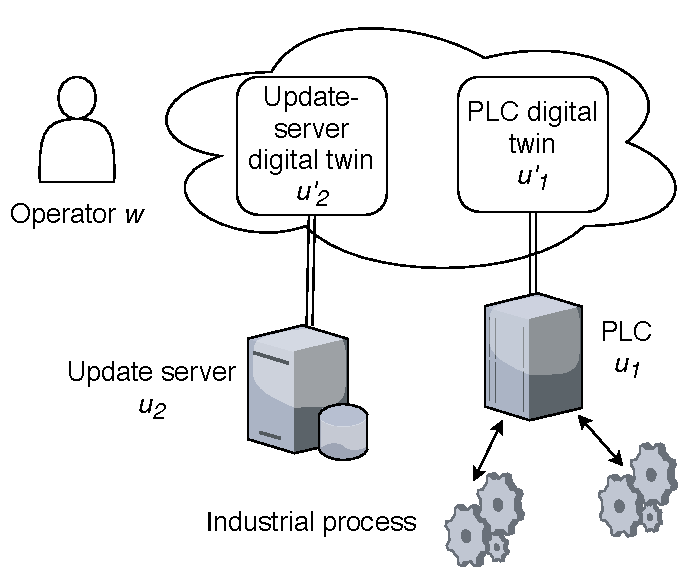
\includegraphics[scale=0.5]{papers/digital-twin/images/FIG7_TII-19-1326}
    \caption{Setup of out digital twin and software update scenario.}
    \label{figure:setup}
\end{figure}

The state information for the supported twins are selected to be: $s_{u'_1} =$ \texttt{[ctrl\_flag, ctrl\_url, sw\_state]} and  $s_{u'_2} = $ \texttt{[ctrl\_url, sw\_package]}\footnote{Here is actually no state information with origin from the physical twin, $u_2$, but just digital twin state information which is propagated to the physical twin.}.  \texttt{ctrl\_flag} is a value holding software upgrade request control and error information and the \texttt{ctrl\_url} is a URL of a new software package to be installed. \texttt{sw\_state} is a list of all current software packages and versions installed on a unit and \texttt{sw\_package} is a new software package.  We also assumes a remote operator, $w$, to be present in the system controlling software upgrades through a remote user device over standard internet. 


\subsection{PLC software update process}
$w$ identifies a new software package, $q$, and connects to the external server $u'_2$.  $w$ then downloads $q$ to $u'_2$ and $w$  receives a \texttt{ctrl\_url} value for the package in return. $u'_2$ then updates the state $\hat{s}_{u'_2,0}$ to reflect the storage of the new software package. Then a synchronization takes place between $u'_2$ and $u_2$. The synchronization is done by sending $\Delta_{\hat{s}_{u'_2}} = $ \texttt{ctrl\_url}$+ q$ from $u'_2$ to $u_2$. This in turn, triggers $u_2$ through the functions $h_{u_2}$ and $z_{u_2}$, to update its internal state, resulting in the storage of $q$ which can be downloaded from \texttt{ctrl\_url} to other units within the local factory network. 

$w$ makes a second request using the newly received \texttt{ctrl\_url} and with information regarding the new software packages towards $u'_1$. The request trigger $u'_1$ to update states $s_{u'_1,1}$: \texttt{ctrl\_flag}, \texttt{ctrl\_url}, \texttt{sw\_state}, where \texttt{ctrl\_flag} contains ''available software update indicator'', \texttt{ctrl\_url} contains the URL to the new software package on $u_2$ and \texttt{sw\_state} contains version information for the pending new software. In the clock cycle 2, this information is propagated to $u_1$ through  $\Delta_{\hat{s}_{u'_1}}$. This values in combination with the functions $h_{u_1}$ and $z_{u_1}$ give an updated state $s_{u_1,2}$.
The SW update flag in state $s_{u_1,2}$ triggers $u_1$ to set the state to update pending allowing to $u_2$ using \texttt{ctrl\_url} to download and install the new SW package, $q$. Once, the update is finalized, the update status information as well as the new SW state information is propagated back to $u'_1$ through updates of the \texttt{ctrl\_flag} and \texttt{sw\_state}.

\vspace*{-0.15in}
\subsection{Performance evaluation}
We have implemented the scenario, described above, with a SW update process using digital twins. As the PLC $u_1$ we have used OpenPLC\cite{Alvares2014}, a free, open source PLC implementation, running on a RaspberryPI\footnote{https://www.raspberrypi.org }. The Raspberry Pi we have used is a model 2 v1.1 with an ARM Cortex-A7 quad-core processor, clocked at 900MHz.

The digital twins $u'_1, u'_2$ are running as separate processes in a Ubuntu 18.04 desktop host. The same host also functions as the update server $u_2$. Since the physical entities synchronize with digital-twins outside the protected factory network the synchronization protocol is secured by DLTS. 

\subsubsection{Update time depending on synchronization frequency}
In order to evaluate the state synchronization protocol we have looked at the SW update scenario. We want to examine how the state synchronization process affects other processes running on the system.

First we ran tests without state synchronization to establish a base line for how long time the update process takes. Then we ran the SW update process with state synchronization at different frequencies. We evaluated performance at 1, 10 and 100 state synchronizations per second. The result can be seen in Fig. \ref{figure:times}\footnote{In the simple system we are using, actually, the state exchange can be omitted in most cases as we very seldom have state changes, but in our evaluation, we anyway forced a state exchange to take place in order to test the synchronization frequency performance impact.}.

As can be seen from the figure the performance impact of the state synchronization is very small. Only at a large number of synchronizations per second is the performance noticeable.
\begin{figure}[ht]
\vspace*{-0.2in}
   \centering
    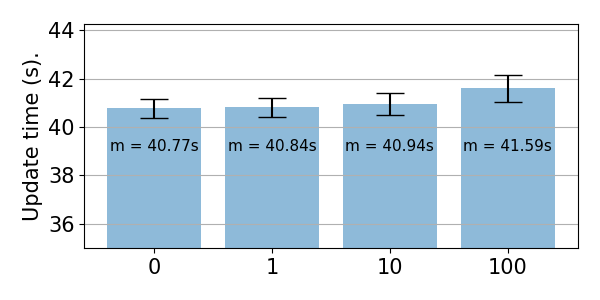
\includegraphics[height=4cm, width=7cm]{papers/digital-twin/images/FIG8_TII-19-1326}
    \vspace*{-0.15in}
    \caption{Update times when using state synchronization at different frequencies.}
    \label{figure:times}
\end{figure}

\subsubsection{Compassion of DTLS Cipher Suites}
We have compared different DLTS cipher suites to evaluate if this impacts performance. The default strong suite AES-256-GCM with SHA384 was compared to the weaker AES-128-GCM with SHA256. The results can be seen in Figure \ref{figure:ciphers}. It can be noted that the choice of ciphers has only a very small impact on the performance of the update process.

\begin{figure}[ht]
\vspace*{-0.2in}
   \centering
    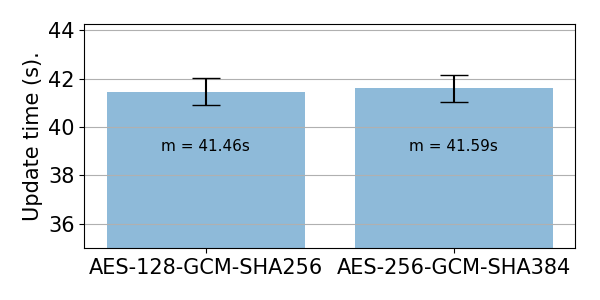
\includegraphics[height=4cm, width=7cm]{papers/digital-twin/images/FIG9_TII-19-1326}
    \vspace*{-0.15in}
    \caption{Comparison of update times with different DTLS cipher-suites.}
    \label{figure:ciphers}
\end{figure}

\subsubsection{Computation cost}
A PLC is not a constrained device in a traditional sense, however, since it controls a time-critical process CPU-time is limited. Any added features must consider this so time-critical deadlines are kept.

We have measured the CPU-time needed by the PLC to implement our state synchronization protocol. By running the protocol over an extended time we have come to the following numbers as seen in Table \ref{table:cpu-time}. 

As shown in the table the CPU-time needed by the PLC to implement the state synchronization protocol is very small. An even slower CPU will still be able to run the state synchronization without overloading the processor.

\begin{table}[]
\begin{tabular}{lll}

 \thead{CPU-time (ms)\\per synchronization} & \thead{ CPU-load  \\ 10 synchronizations/s} & \thead{CPU-load \\ 100 synchronizations/s} \\ \hline
           $0.3772 \: (s = 0.0602)$   & $0.0038\%$   &   $0.0377\%$                       \\ 
\end{tabular}
\caption{Measurements of CPU-time per state synchronization message and CPU-load.}
\label{table:cpu-time}
\end{table}
% 900mhz 4 cors  



\subsubsection{Network performance}
Evaluating network performance for the state synchronization process is difficult to do without real ICS network traffic to base an evaluation scenario on. Hence, instead we evaluated the performance in an isolated system. We measured the bandwidth consumption for the PLC during the update process. We then measured the bandwidth for the update process while synchronizing with the PLC's digital-twin. The synchronization messages were of size 22 bytes in each direction. The bandwidth consumption can be seen in Table \ref{table:network-overhead}. As can be seen from the Table the bandwidth consumption is reasonable for small synchronization frequencies.

\begin{table}[]
\begin{tabular}{l|l|l}
    & Bandwidth to PLC & Bandwidth from PLC \\ \hline
No synch  &     0.97 KB/s      &     2.06 KB/s    \\
1 synch/s &     1.20 KB/s       &    2.38 KB/s   \\
10 synch/s &      2.16 KB/s     &     3.35 KB/s        \\
100 synch/s &     10.88 KB/s     &    12.06 KB/s

\end{tabular}
\caption{Bandwidth to and from the PLC when updating.}
\label{table:network-overhead}
\end{table}


\iffalse
\begin{table}[]
\begin{tabular}{l|l|lll}
    Message Length & Synchronization  & \multicolumn{3}{l}{Devices on network} \\
                                &  frequency                                   & 1           & 10         & 100         \\ \hline
\multirow{3}{*}{20}             & 1                                   & 40B/s       & 400B/s     & 4KB/s       \\
                                & 10                                  & 400B/s      & 4KB/s      & 40KB/s      \\
                                & 30                                  & 600B/s      & 6KB/S      & 60KB/s      \\
\multirow{3}{*}{50}             & 1                                   & 100B/s      & 1KB/s      & 10KB/s      \\
                                & 10                                  & 1KB/s       & 10KB/s     & 100KB/s     \\
                                & 30                                  & 3KB/s       & 30KB/s     & 300KB/s    
\end{tabular}
\caption{Network usage for different sizes of synchronization messages, synchronization frequencies and number of devices on network.}
\label{table:network-overhead}
\end{table}
\fi

\section{Conclusion and future work}
\label{sec:digital-twin:conclusion}
Motivated by the need for new security models and principles in IACS to open up the systems for cloud based processing and data sharing, we investigated how digital twins can work as a security enablers in IACS. We introduced a new adversary model, made basic security definitions, identified security requirements, made a novel security architecture and in particular state replication design for a digital twin based IACS. The new state replication design as well as the architecture were then security evaluated against the identified requirements. We showed that the proposed synchronization design meets the introduced digital twin synchronization requirements. Furthermore, we made a high-level design of the other security components in the architecture and argue about how the suggested functions will help in meeting the identified security requirements.  Through our proof of concept implementation and performance evaluation, we also showed that the new digital twin synchronization model works well in practice for a small but real production case with reasonable performance impact. Especially, we show that as long as we have not too high update frequency, the performance impact on a platform like RaspberryPI is negligible. As expected, the bandwidth increases linear with the synchronization frequency. In our evaluation, we only reflected a few PLC states, and obviously, the more fine grain states that are reflected, the more impact it will have on the system performance and bandwidth consumption.

The results shows that a digital twin based security architecture can be a promising way to protect IACS while open them up for external data sharing and access. We have here worked with defining a suitable overall architecture and synchronization model. In order to develop a fully working system based on our architecture and approach, more work is needed. Below, we discuss the most important future work:
\begin{itemize}
\item \textbf{Performance:} We have here made first proof of concept of the architecture. In order to see the effect of the architecture on different platform and production scenarios, more performance evaluations on different platform, with more complex digital twin state models and with larger amount of production nodes are needed. 
\item \textbf{Intrusion detection:} In our security architecture, we have only show how on principle level how  to integrate intrusion detection at the boarder to the virtual domain. It is left for future research to design and integrate intrusion detection in a fully working system.
\item \textbf{Access control:} The architecture allows for advanced access control in the virtual domain. The main advantage with this approach is that this can be supported without affecting the production domain at all. It remains to design and evaluate this approach in a full system implementation of the architecture.
\item\textbf{Formal security analysis:} We have proven the consistency of the proposed synchronization protocol and showed that the security of the protocol depends on the security of the underlying used secure channel. Formal analysis of the security of the complete system design and all protocols are left for future work. 
\item \textbf{Security analysis services:} Apart from IDS and access control enforcement in the virtual domain, additional security analysis services may be supported as virtual components as we showed in our architecture design. This include services such as virus scan, DoS prevention etc. The design and evaluation of such services is left to future research as well.
\end{itemize}

\section*{Acknowledgement}
We would like to thank the SSF SEC4FACTORY project team for valuable discussions regarding the research direction and results presented in the paper. In particular we would like to thank the TetraPak project members for their valuable feedback and suggestions.

{\raggedright
        \printbibliography[segment=\therefsegment,heading=subbibliography]
}

